%%%%%%%%%%%%%%%%%%%%%%%%%%%%%%%%%%%%%%%%%%%%%%%%%%%%%%%%%%%%%%%%%%%%%%%%%%%%%%%%
%2345678901234567890123456789012345678901234567890123456789012345678901234567890
%        1         2         3         4         5         6         7         8

%\documentclass[letterpaper, 10 pt, conference]{ieeeconf} % Comment this line out if you need a4paper

\documentclass[a4paper, 10pt, conference, twocolumn]{ieeeconf}       % Use this line for a4 paper

\IEEEoverridecommandlockouts                              % This command is only needed if 
                                                          % you want to use the \thanks command

\overrideIEEEmargins                                      % Needed to meet printer requirements.

%In case you encounter the following error:
%Error 1010 The PDF file may be corrupt (unable to open PDF file) OR
%Error 1000 An error occurred while parsing a contents stream. Unable to analyze the PDF file.
%This is a known problem with pdfLaTeX conversion filter. The file cannot be opened with acrobat reader
%Please use one of the alternatives below to circumvent this error by uncommenting one or the other
%\pdfobjcompresslevel=0
%\pdfminorversion=4

% See the \addtolength command later in the file to balance the column lengths
% on the last page of the document

% The following packages can be found on http:\\www.ctan.org
%\usepackage{graphics} % for pdf, bitmapped graphics files
%\usepackage{epsfig} % for postscript graphics files
%\usepackage{mathptmx} % assumes new font selection scheme installed
%\usepackage{times} % assumes new font selection scheme installed
%\usepackage{amsmath} % assumes amsmath package installed
%\usepackage{amssymb}  % assumes amsmath package installed
\usepackage{cite}
\usepackage[UTF8]{ctex} 
\usepackage{graphicx}
\usepackage{amsmath}

\title{\LARGE \bf
Automatically Fixing Vulnerabilities in WebAssembly
}


\author{Yubin Hu$^{1}$ % <-this % stops a space
% \thanks{*This work was not supported by any organization}% <-this % stops a space
% \thanks{$^{1}$Albert Author is with Faculty of Electrical Engineering, Mathematics and Computer Science,
%         University of Twente, 7500 AE Enschede, The Netherlands
%         {\tt\small albert.author@papercept.net}}%
% \thanks{$^{2}$Bernard D. Researcheris with the Department of Electrical Engineering, Wright State University,
%         Dayton, OH 45435, USA
%         {\tt\small b.d.researcher@ieee.org}}%
}


\begin{document}


\maketitle
\thispagestyle{empty}
\pagestyle{empty}


%%%%%%%%%%%%%%%%%%%%%%%%%%%%%%%%%%%%%%%%%%%%%%%%%%%%%%%%%%%%%%%%%%%%%%%%%%%%%%%%
\begin{abstract}

Unlike Ethereum, the EOSIO blockchain platform is unique in that the features and characteristics of the blockchain built on it are flexible, which means they can be changed and modified completely to suit business case requirements.
Thus, many developers update the code when bugs are detected.
In this paper, we propose a method to find security issues of EOSIO smart contracts by comparing the history version.
After analyzing all the security issues in EOSIO smart contracts,
we integrate the causes, patterns, and solutions to the security issues.
Eventually, we will explore how to automatically fix vulnerabilities in smart contracts.

\end{abstract}


%%%%%%%%%%%%%%%%%%%%%%%%%%%%%%%%%%%%%%%%%%%%%%%%%%%%%%%%%%%%%%%%%%%%%%%%%%%%%%%%
\section{Introduction}

The EOSIO is the most popular public blockchain platform supporting smart contracts and has grown rapidly in recent years.
As of 2019, the total value of on-chain transactions of EOSIO has exceeded 6 billion USD.
Furthermore, EOSIO is still in its early stages and has some experimental characteristics.
As a result, as new bugs and security are discovered and new features are developed, the security threats we face constantly change.
The vulnerabilities within smart contracts have led to severe financial loss.
EOS Bet — a gambling dApp which uses EOS tokens, lost at least \$338,000 from its operational wallets to hackers on 2018-10-15\cite{medium:2018}.

Therefore, we need practical vulnerability detection tools to safeguard the ecosystem of blockchain.
However, the vulnerability detection tools for EOSIO smart contracts are limited.
EOSAFE\cite{272292} and WANA\cite{Wang2020WANASE} support detecting specific bugs, such as Fake EOS, Fake Receipt, Rollback, and Missing Permission Check.\cite{eosio}
Although the current detection effect has reached the expected level, it will not have a good effect on new vulnerabilities or some artificially maliciously implanted vulnerabilities.

WebAssembly (abbreviated Wasm) is a binary instruction format for a stack-based virtual machine.
On top of the EOSIO core layer, a WebAssembly virtual machine, \emph{EOS VM}, executes smart contract code, and it is designed from the ground up for the high demands of blockchain applications which require far more from a WebAssembly engine than those designed for web browsers or standards development.
The EOSIO smart contracts are developed using cpp or rust.
And they can be compiled into WebAssembly code for execution in the corresponding WebAssembly VM implementation with \emph{eosio.cdt} (EOSIO Contract Development Toolkit)

For Ethereum, the only way to destroy a smart contract on the blockchain system is using the \emph{Selfdestruct} function when attackers find the bugs.
Unlike Ethereum, applications deployed on EOSIO-based blockchains are upgradeable.
This means you can deploy code fix, add features, and change the application’s logic as long as sufficient authority is provided.
As a developer, you can iterate your application without the risk of being locked into a software bug permanently.
We can easily collect several versions of the same smart contract.
Generally speaking, the code updated by the developer may be vulnerabilities, new functions, or even artificially implanted code with fraud.

This paper first crawls all the verified (open-sourced) smart contracts with several versions from EOSIO.
Then we compare the differences between different versions of the same smart contract from the symbolic execution path.
Finally, we analyze the differences to summarize the security issues and other reasons for smart contract updates.

\section{Backgroud}


\subsection{WebAssembly}

WebAssembly (abbreviated Wasm) is a binary instruction format for a stack-based virtual machine.
Wasm is designed as a portable compilation target for programming languages, enabling deployment on the web for client and server applications\cite{webassembly}.
The WebAssembly virtual machines can be embedded into Web browsers or blockchain platforms. The EOSIO blockchain has supported Wasm.
Furthermore, in Ethereum 2.0, Wasm VM is the replacement of Ethereum VM (EVM).

The design choice of using Wasm enables EOSIO to reuse optimized and battle-tested compilers and toolchains which are being maintained and improved by a broader community.
In addition, adopting the Wasm standard also makes it easier for compiler developers to port other programming languages onto the EOSIO platform.

There are two convertible and equivalent representations for WebAssembly.
We have a binary format - ".wasm" as the suffix.
To enable WebAssembly to be read and edited by humans, there is a textual representation of the Wasm binary format - ".wast" as the suffix.

\subsection{EOSIO}

EOSIO is a free, open-source blockchain software protocol that provides developers and entrepreneurs with a platform on which to build, deploy and run high-performing blockchain applications.

\subsubsection{Accounts}

An \emph{account} is a human-readable name stored on the blockchain\cite{eosio}.
In order to ensure account security and prevent identity fraud, EOSIO has implemented an advanced access control system based on permissions.
An \emph{account} is required to transfer or push any valid transaction to the blockchain.

\subsubsection{Delegated Proof of Stake (DPOS)}

The EOSIO platform implements a proven decentralized consensus algorithm capable of meeting the performance requirements of applications on the blockchain called the \emph{Delegated Proof of Stake} (DPOS).
Under this algorithm, if you hold tokens on a EOSIO-based blockchain, you can select block producers through a continuous approval voting system.
Anyone can choose to participate in the block production and will be allowed to produce blocks, provided they can persuade token holders to vote for them\cite{eosio}.

\subsubsection{Smart Contracts}\label{2.2.3}

\textbf{Smart contract} is a piece of code that can execute on a blockchain and keep the state of contract execution as a part of the immutable history of that blockchain instance.
Therefore, developers can rely on that blockchain as a trusted computation environment in which inputs, execution, and the results of a \emph{smart contract} are independent and free of external influence.
Every EOSIO smart contract must use \emph{apply} functions as input functions to process operation.

\textbf{Transactions} are composed of one or more actions, which are the basic units for triggering functions in smart contracts.

\textbf{Dispatcher} When one account needs to adjust the smart contract of another account, and the smart contract needs to be processed and dispatched, then we need a dispatcher.

\begin{figure}[h]
    \centering
    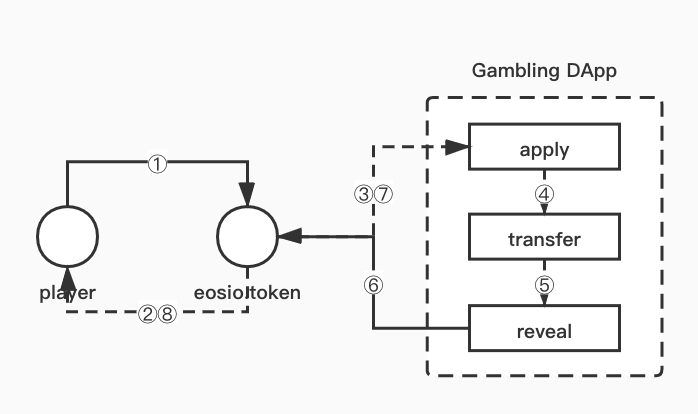
\includegraphics[width=0.4\textwidth]{figures/life-cycle.jpg}
    \caption{life-cycle of smart contract execution\cite{272292}\cite{eos:transactions_protocol}}
\end{figure}

The life-cycle of smart contract execution\cite{272292}:
\begin{enumerate}
    \item Invoke transfer to take part in game
    \item Notify player (payer)
    \item Notify DApp (payee)
    \item Dispatch to transfer function
    \item Invoke reveal to calculate jackpot
    \item Invoke transfer to return prize
    \item Notify DApp (payer) 
    \item Notify player (payee)
\end{enumerate}

In this process, due to various reasons, such as failing to check the authentication parameters, security issues will occur.

\section{Vulnerabilities}

\subsection{Fake EOS}\label{3.1}
\textbf{Cause of vulnerability} 
In EOSIO smart contract,
we need \emph{EOS} token at the 3rd step of the generate life-cycle of smart contract execution.
However,
anyone, including a hacker, can create a token through the public code of EOSIO.token.
And the name of the token can be repeated.
This means that the name of the token created by the hacker can also be called \emph{EOS}.

Generally speaking, a hacker creates an \emph{EOS} token and name is \emph{EOS},
then transfer the amount of these fake EOS tokens to a EOSIO smart contract.
If the DApp’s code is robust enough,
then the hacker’s attack should have failed.
Although the name is the same as the real EOS token,
the issuer is different.
The hacker transmits the EOS token to the DApp through the copy, and then the DApp will not receive the notified \emph{code} EOS token.
If it happens that the DApp does not check the value of the \emph{code} at this time,
the verification of the dispatcher will be bypassed.

In order to avoid the above problems as much as possible,
developers simply narrowed the scope of accepting code,
but it can also be bypassed.
Obviously, this approach is not rigorous enough.
It is this place that gives us the possibility of detecting vulnerabilities.

\textbf{Harm of vulnerability}
Early morning on 2018-10-31,
online media reported that gambling platform EOSCast was attacked by hackers and lost more than 70K EOS tokens.\cite{peckshield:2018}

\subsection{Fake Receipt}\label{3.2}
\textbf{Cause of vulnerability} 
In the generate life-cycle of smart contract execution,
the notification will be forwarded when the developer checks the \emph{code}.
Also, notification can be forwarded by the dispatcher even the code will not be changed.
This is the key to this vulnerability being attacked.

Hackers play two roles in this game,
and one is \emph{initiator}, the other is \emph{accomplice}.
The initiator invokes a \emph{transfer} to the accomplice through the EOS token.
When the EOS token notifies the accomplice,
the code is not changed and is directly forwarded to the DApp.
However, if the parameters are not checked during \emph{transfer},
the EOS token will be passed between the two roles of the hacker,
which will lead to EOS loss.

\subsection{Rollback}\label{3.3}
\textbf{Cause of vulnerability} 
The transaction can be rolled back in some malicious ways,
which is not a good thing for some gambling DApps.
Suppose that in the gambling DApp,
in the generate life-cycle of smart contract execution,
when the eighth step, "Notify player" is executed,
the hacker can immediately check whether the EOS balance of his account has decreased.
If it reduces,
the hacker will immediately call the interrupt to roll back the gambling.
Such gambling is meaningless, and hackers will always win.

\textbf{Harm of vulnerability}
On the day 2018–12–19,
Most of the gambling dapp was suffered rollback attack,
including Betdice, EOSMax, Tobet, etc.
Caluclating at the price of 18 RMB each EOS,
it had loss over 500 million rmb.\cite{slowmist:2019}

Through the transaction records of the account, we can find that the account has only revealing records and no betting records.

\subsection{Missing Permission Check}\label{3.4}
\textbf{Cause of vulnerability} 
In the generate life-cycle of smart contract execution,
the fifth step, "Invoke reveal to calculate jackpot",
the DApp should check whether the caller is actually the payer.
We have such a function \emph{require\_auth()\*} in EOSIO,
it is used to check whether the caller is authorized to call some methods.
There is a pre-knowledge here,
inlined actions inherit the permissions of the father.
Therefore, hackers can execute inlined actions by calling functions to perform operations that the hacker does not have the authority to perform,
which leads to security problems.

\subsection{Reentrancy}

In July 2016, a fault in TheDAO contract allowed an attacker to steal \$50M.
The atomicity and sequentiality of transactions may make developers believe that it is impossible to re-enter a non-recursive function before its termination. However, this belief is not always true for smart contracts

First, the $attack()$ function in the attacker contract is called, which deposits some ethers in the victim contract and then invokes the victim’s vulnerable $refund()$ function.
Then, the $refund()$ function sends the deposited ethers to the attacker contract, also triggering the unnamed fallback function in the attack contract.
Next, the fallback function again calls the $refund()$ function in the victim contract.
Since the victim contract updates the userBalances variable after the ether transfer call, userBalances remains unchanged when the attacker re-enters the $refund()$ function, and thus the balance check can still be passed.
As a consequence, the attacker is able to repeatedly siphon off ethers from the victim contract and exhaust its balance

\subsection{Missing Input Validation}

The arguments of a function should be validated before their uses. 
If developers forget to assign correct values to the arguments, EVM will execute the function using the default values based on the argument types.
This mechanism makes smart contracts vulnerable to the attacks on function arguments.

\subsection{Unhandled Exception}
In Solidity, there are multiple situations where an exception may be raised. Unhandled exceptions can affect the security of smart contracts. 
In February 2016, a vulnerable contract forced the owner to ask the users not to send ether to the owner because of an unhandled exception in the call instruction.

\subsection{Arithmetic Vulnerability}

Arithmetic vulnerability is a common bug, and it is no exception on smart contracts.
Integer overflow vulnerabilities and divide-by-zero vulnerabilities are all vulnerabilities that need to be focused on.

\subsection{Feasibility \& Versatility}

\begin{figure}[h]
    \centering
    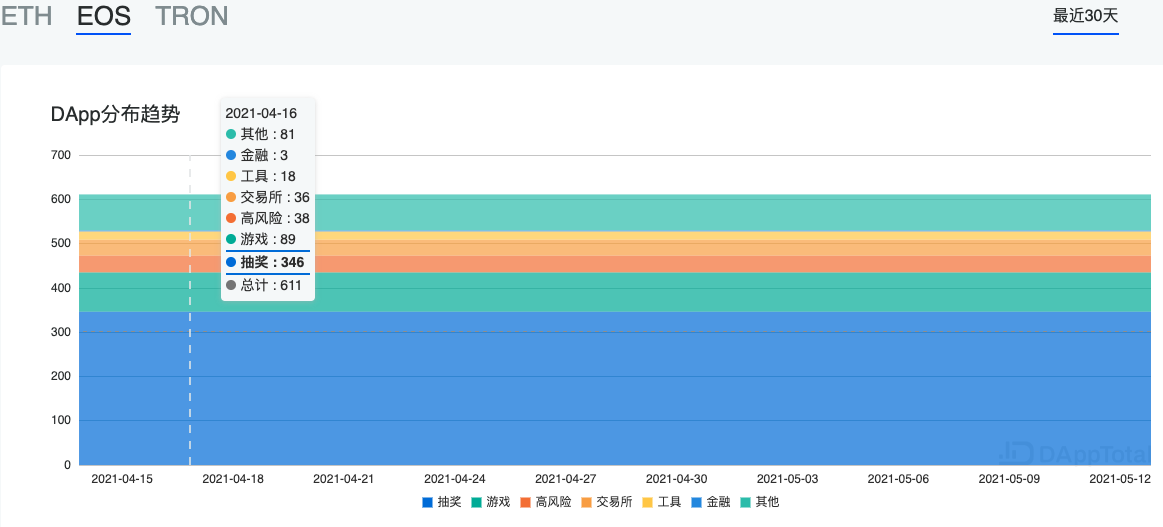
\includegraphics[width=0.4\textwidth]{figures/dapptotal.png}
    \caption{DApp distribution trend. \\ From the figure, we can see that in 2021-04-16, out of a total of 611 DApps, 346 DApps are of the gambling type, and 89 DApps are of the game type.}
\end{figure}

The above four vulnerabilities are common problems that may exist in EOS smart contracts,
rather than special cases.
According to research in EOSafe, 88.32\% of EOSIO smart contracts are deployed using the transfer function.
And Fake EOS and Fake receipt need to use the transfer function.
Although Rollback is only found in gambling games,
from the perspective of DappRadar\cite{DappRadar} and DAppTotal\cite{DAppTotal},
gambling games are the most popular Dapp.
And Missing Permission Check is a common and high-risk vulnerability.

\section{Research Questions}


\subsection{Differences Between History Version}

We aim to compare the differences between different versions of the same smart contract.
So we are thinking about how to visually and effectively analyze the difference between the two codes.

\subsubsection{Compare Codes Line By Line}
Compare codes line by line is not a good choice. First,
our code is in wasm bytecode format, which is not conducive to reading.
Even if converted to wat format,
it isn't easy to get specific meaning from the surface for codes similar to assembly language.
So obviously, we will not take this approach.

\subsubsection{Control Flow Graph}
The control flow graph is an abstract representation of a process or program.
It is an abstract data structure used in the compiler.
It is maintained internally by the compiler and represents all the paths traversed during the execution of a program. It expresses the possible flow of execution of all basic blocks in a process in the form of a graph
and can also reflect the process's real-time execution process.

\subsubsection{Sybolic execution path}

\begin{figure}[h]
    \centering
    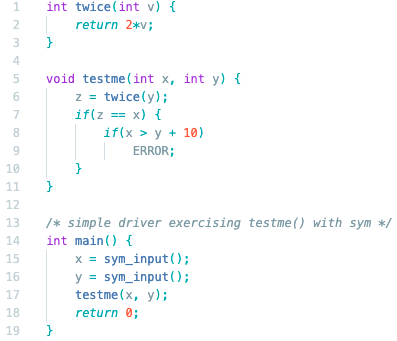
\includegraphics[width=0.5\textwidth]{figures/sym_code.png}
    \caption{Sybolic Code Example}
\end{figure}
\begin{figure}[h]
    \centering
    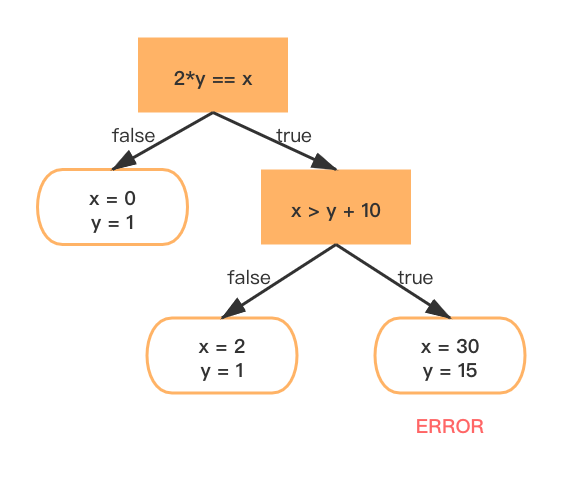
\includegraphics[width=0.5\textwidth]{figures/sym_graph.jpg}
    \caption{Sybolic Execution Tree}
\end{figure}

Symbolic execution is a means of analyzing a program to determine what inputs cause each part of a program to execute.
An interpreter follows the program,
assuming symbolic values for inputs rather than obtaining actual inputs as normal execution of the program would.
It thus arrives at expressions in terms of those symbols for expressions and variables in the program,
and constraints in terms of those symbols for the possible outcomes of each conditional branch.

The path constraint generated by symbolic execution makes it easier for us to detect the difference between the two codes.

\subsection{Path Explosion}\label{4.2}
There are two instructions for branch jump in EOSIO,
\emph{br\_if} and \emph{br\_table}. \emph{br\_if} will generate two branches.
And \emph{br\_table} takes a vector of an arbitrary number \emph{n} of label indices as its first immediate,
and another label index as its second immediate.
This means that \emph{br\_table} can generate \emph{n} branches.
Once the code has a deep call stack, the complexity of program analysis will increase exponentially.\cite{272292}

Under the framework of EOSafe,
it has used heuristic pruning to try to solve the above problems,
and added \emph{call\_depth} to limit the call depth. On this basis,
we only focus on some critical functions,
and other functions that have little impact on our research content can be ignored.

Finally, set the timeout period to prevent the analysis from being unable to continue due to excessive code complexity.

\subsection{Automatic Fixes}

When a vulnerability is detected, the focus of attention is on how to automatically fix the vulnerability.

Automated repair of vulnerabilities in smart contracts poses unique challenges to existing repair techniques.
First, existing repair techniques rely heavily on test suites to detect incorrect program behavior and to validate the generated patches.
However, test suites that are difficult to obtain, if not impossible, to address all vulnerabilities are difficult, if not impossible, to obtain, resulting in generated patches that do not fix vulnerabilities.
Second, by utilizing search algorithms such as genetic programming or random search using search algorithms, existing repair techniques explore the repair space based on syntax mutators.
However, the repair strategies of these techniques, which mainly add conditional checks or replace a statement with another existing statement, are not sufficient to repair intelligent contracts that require temporary variable creation and statement reordering (e.g., repairing re-entrant vulnerabilities).
Moreover, simply adapting these techniques to include more complex fixing strategies can easily lead to an exponential expansion of the search space.
Third, applying patches beyond adding conditional checks may change the semantics of smart contracts and even introduce new code faults or vulnerabilities.

\section{System Design}


For this stage, we collect data for the following stages.
We crawl the verified smart contracts, which are the open-sourced contracts.
We have synchronized the EOS mainnet nodes.
The complete history node provides an analysis layer on top of historical data,
making DApp easier to process and use.
In order to process this type of data, nodes need to run full history plugins and solutions,
which require a lot of RAM and high maintenance costs.
DApp developers can use the complete history node to track and query the data of a specific user account,
and we can extract all operations or transactions associated with a specific account to obtain every update of a specific smart contract.

Although there are some public EOS data sets on the Internet,
we need the special data required for the experiment which are different versions of the same smart contract.
And only the code API of the requesting node cannot get the historical information,
it only returns the latest code.
So we need to filter out the EOSIO `setCode` action, grab all the `setCode` information of the related account, then parse the data packet, and get the Wasm code through decoding.

But there are too many node history records,
and there are many repetitive data,
it isn't very meaningful for the experiment.
So we chose to use the records before 2019-03-27,
the data volume is top 50 million blocks,
and the size is about 91GB.

\subsection{Difference comparison}
First, we select the cleaned data and choose EOSIO smart contracts with multiple versions.

Then, among multiple versions,
we select two adjacent versions in turn for different analysis.
The reason why two adjacent versions are chosen instead of any two versions is that one is that the number of codes to be compared increases,
and the other is that the code modification of the two adjacent versions can best reflect the modified content.
If the old version contains vulnerabilities and the new version fixes the vulnerabilities,
we can clearly determine the type of vulnerabilities and how to fix them by analyzing the differences between the two codes.

After the two versions of the code are selected,
emulate the code is executed,
and the control flow diagram and symbolic execution path of the two versions are produced respectively.
The control flow graph is convenient for experimenters to observe the difference of the code visually,
and the symbolic execution path and some recorded states are used to automatically analyze whether there are vulnerabilities and the types of vulnerabilities.

We have implemented three types of vulnerability detectors in the experiment.
They are Fake EOS Detector, Fake Receipt Detector,
and Missing Permission Check Detector.
The reason why the Rollback detector is not implemented is that the detection complexity of the rollback is extremely high.
Generally, one can only try to substitute a particular method to perform the detection.
Due to the time factor,
the Rollback detector is temporarily not implemented.

\subsection{Frame}
We use Octopus and EOSafe as framework.
Octopus is a security analysis framework for WebAssembly module and Blockchain Smart Contract.
The purpose of Octopus is to provide an easy way to analyze closed-source WebAssembly modules and smart contracts bytecode to understand deeper their internal behaviors.


\section{Vulnerabilities Dectection}


\subsection{Fake EOS Detector}
According to the life-cycle of smart contract execution in \ref{2.2.3} and the cause of the Fake EOS vulnerability we know in \ref{3.1},
we found that the smart contract containing the vulnerability of Fake EOS must be called by the hacker to transfer the function,
and successfully bypassed the code. An examination.
Then we only need to perform symbolic execution on the apply function,
generate a symbolic execution path,
and determine whether the difference constraints between the new and the old version is:

\begin{equation}
\begin{aligned}
action == transfer,(\rm~in~apply~function) \\ \bigwedge~code == account~name,~not~self,(\rm~in~apply~function) 
\end{aligned}
\end{equation}

If the new and old versions of the EOSIO smart contract meet the above conditions,
we will consider the old version of the EOSIO smart contract to be fragile and may contain the vulnerability of Fake EOS,
and it has been fixed in the new version.

We only need to analyze the differences in the paths related to transfer,
and the differences in other paths will hardly cause Fake EOS.
This is a direction that can be optimized for pruning.

\subsection{Fake Receipt Detector}
According to the life-cycle of smart contract execution in \ref{2.2.3} and the cause of the vulnerability of Fake Receipt we know in \ref{3.2},
we found that the critical factor of the smart contract that contains the vulnerability of Fake Receipt is insufficient verification in the transfer function.
Then our approach is straightforward: find all the functions that may call/jump to the transfer function,
perform symbolic execution, generate a symbolic execution path,
and determine whether there are operations to modify the state of the blockchain between the new and old versions of the suspicious functions,
and whether there is a function such as \emph{eosio\_assert()} to interrupt the path that does not jump.

\begin{equation}
\begin{aligned}
self==to,~modification,(\rm~in~suspicious~function) \\
\bigwedge~self!=to,~eosio\_assert(),(\rm~in~suspicious~function) 
\end{aligned}
\end{equation}

\subsection{Missing Permission Check Detector}

According to the life-cycle of smart contract execution in \ref{2.2.3} and the cause of the Missing Permission Check vulnerability we know in \ref{3.4},
we only need to pay attention to whether functions check permissions before performing sensitive operations.
And all functions are connected with apply function in the call graph.
So we can perform symbolic execution on the apply function,
find all functions, and check whether a permission check has been added before the instructions for some sensitive operations that we have counted.
If permission check is added,
we can think that the old version of EOSIO smart contract has the Missing Permission Check vulnerability,
and it has been fixed in the new version.

\begin{equation}
\begin{aligned}
sensitive~operations == db\_update_i64(\*), etc. \\
\exists sensitive~operations \bigwedge no~require\_auth(\*)
\end{aligned}
\end{equation}

\section{Automatic Fixes}

In this section, we present the fix patterns used for patch generation.
Our program analysis supports fix patterns in three granularity levels: statement level, method level, and contract level.
Next will be a description of the vulnerabilities that can be fixed and how to generate patches.

\subsection{Reentrancy}

The preferred fix pattern for Reentrancy is to move all writes to storage ahead so that there is no write to storage after an external method call or a coin transfer call.

\subsection{Missing Input Validation}

The fix pattern for MissingInputValidation is to add conditional checks to validate the method parameters at the beginning of method body.

\subsection{Unhandled Exception}

The fix pattern for this vulnerability is to check the return value of each call statement.
Program adds a $require()$ function call to validate the return values of $send()$ and $value()$ and ensures that their executions are successful before completing the whole transaction.

\subsection{Algorithm vulnerability}

The fix for the arithmetic vulnerability is to replace all unsafe arithmetic functions with safe ones.

\section{Evaluation}

\subsection{Dataset}
We use the EOSIO records before 2019-03-27,
the data volume is top 50 million blocks.
In the data set after data cleaning,
there are \emph{1373} smart contracts,
and \emph{610} smart contracts have multiple versions.
There are \emph{2849} pairs of old and new version codes in total.

\subsection{The Accuracy of Vulnerability Detection}
In order to evaluate the detection level of this system,
we inquired about the reports issued by blockchain security companies such as PeckShield\cite{peckshield:2020} and SlowMist\cite{slowmist:2020} to confirm that the vulnerabilities we found were accurate and real.
And at the same time, use EOSafe to assist judgment. EOSafe is an excellent detection framework.
In its previous experiments,
its precision and recall were 100\% and 96.30\%,
respectively. We believe that EOSafe can serve as an effective referee.

Through comparison,
we found that EOSIO smart contracts with vulnerabilities detected by this system can all be confirmed on EOSafe.
However, there is a phenomenon of underreporting in this system,
and the general reasons are as follows:
\begin{itemize}
    \item The timeout setting time is relatively short, resulting in \emph{587} EOSIO smart contracts that cannot be fully analyzed (the three detectors cannot be successfully executed within the specified time).
    \item The detection conditions of the detector need to be strengthened.
    \item Because the data is the first 50 million blocks, and the last block is dated 2019-03-27, EOSIO has just developed, many vulnerabilities have not been discovered, and no developers have fixed these blockchain security issues, so there are a lot of historical version codes. Both have the same problem, and it is impossible to check out the vulnerabilities by comparing the differences.
\end{itemize}

\subsection{Distribution of vulnerabilities}

\begin{table}[htp]
    \centering
    \begin{tabular}{|l|l|l|}
    \hline
    Type                     & \# Candidates & \# Vulnerable (\%) \\ \hline
    Fake EOS                 & 23            & 1(4.35\%)           \\
    Fake Receipt             & 23            & 2(8.70\%)           \\
    Missing Permission Check & 23            & 4(17.39\%)          \\ \hline
    Total                    & 23            & 7(30.43\%)          \\ \hline
    \end{tabular}
    \caption{Vulnerabilities Detection Result. \\
    Candidates are smart contracts that can run under specified time and conditions. 
    Vulnerable (\%) is the proportion of smart contracts that have vulnerabilities in the smart contracts that are detected.}
\end{table}

Since there are multiple versions in an EOSIO smart contract,
as long as there is a pair of old and new versions of the code and vulnerabilities are detected,
we can consider the EOSIO smart contract to be fragile and insecure.
We found that among the EOSIO smart contracts that can fully execute the 3 vulnerability detectors,
30.43\% of the smart contracts have security issues.
The most frequent problem is Missing Permission Check,
followed by Fake Receipt,
and the least one is Fake EOS.

Among the smart contracts in the data set,
the smart contract with the most historical versions is guydgnjygige,
a popular gaming platform.
Of course it also has the most vulnerable versions.

By manually inspecting the EOSIO smart contract for which vulnerabilities were detected,
we found the following problems:
\begin{enumerate}
    \item The vulnerabilities repaired by DApp developers are generally very fast. For example, the smart contract danakilblock introduced the vulnerability at 2018-09-05T 19:41:37.500, and updated the version at 2018-09-05T 20:00:42.000 to solve the Missing Permission Check.
    \item When DApp developers update the code, they may fix vulnerabilities in the code and update the business code more often. Of course, as long as the code is updated, new vulnerabilities are likely to be introduced. According to our manual inspection, there are two EOSIO smart contracts that have not been detected vulnerabilities in the old version, but were detected after updating the business code. This reminds DApp developers to avoid creating new vulnerabilities as much as possible when developing new features.
    \item After relevant blockchain security companies released security reports, DApp developers updated smart contracts more intensively.
\end{enumerate}

\subsection{Automatic Fixes result}

Automatic fixes for Arithmetic Vulnerability, Unhandled Exception, Missing Input Validation vulnerability can solve the original problem.
However, more work needs to be done on other vulnerabilities such as reentrant vulnerabilities.

\section{Conclusions}

In this paper,
we proposed the idea of searching for security issues in EOSIO smart contracts by comparing historical versions,
and implemented three types of vulnerability detectors.
Finally automatic fixes were made for specific vulnerabilities.
According to the experimental results,
in the current EOSIO ecological environment,
there are still many smart contracts facing the situation of being exploited by hackers to obtain illegal benefits.
Our research results have further verified that EOSIO's blockchain security needs to be improved.

\addtolength{\textheight}{-12cm}   % This command serves to balance the column lengths
                                  % on the last page of the document manually. It shortens
                                  % the textheight of the last page by a suitable amount.
                                  % This command does not take effect until the next page
                                  % so it should come on the page before the last. Make
                                  % sure that you do not shorten the textheight too much.

%%%%%%%%%%%%%%%%%%%%%%%%%%%%%%%%%%%%%%%%%%%%%%%%%%%%%%%%%%%%%%%%%%%%%%%%%%%%%%%%




%%%%%%%%%%%%%%%%%%%%%%%%%%%%%%%%%%%%%%%%%%%%%%%%%%%%%%%%%%%%%%%%%%%%%%%%%%%%%%%%
% \section*{APPENDIX}

% Appendixes should appear before the acknowledgment.

% \section*{ACKNOWLEDGMENT}

% The preferred spelling of the word acknowledgment in America is without an e after the g. Avoid the stilted expression, One of us (R. B. G.) thanks . . .  Instead, try R. B. G. thanks. Put sponsor acknowledgments in the unnumbered footnote on the first page.\cite{236260}
%%%%%%%%%%%%%%%%%%%%%%%%%%%%%%%%%%%%%%%%%%%%%%%%%%%%%%%%%%%%%%%%%%%%%%%%%%%%%%%%


% \begin{thebibliography}{99}
% \end{thebibliography}


\bibliographystyle{ieeetr}
\bibliography{BibTeX.bib}


\end{document}